\chapter{Acoplamiento de modos $p_y$ y ángulo de invisibilidad}

En electrostática, es posible describir las interacciones dipolares eléctricas mediante los polinomios de Legendre de orden 2, $P_2(\cos\theta) = 3\cos^2\theta - 1$, donde $\theta$ representa el ángulo entre los dipolos. El valor $\theta_m \approx 0.62$ radianes se denomina \textit{ángulo mágico}, ya que anula el término de interacción dipolar \citep{medmagic}.

Este capítulo se centra en los llamados modos $p_y$ o modos dipolares verticales, cuya excitación requiere superar la condición de corte (longitud de onda suficientemente pequeña junto con un contraste $\Delta n$ y un ancho de guía suficientemente grandes).

\section{Acopladores}

Al estudiar el acoplamiento entre modos $p_y$ en guías elípticas, se distinguen dos casos límite:
\begin{enumerate}
    \item Para acopladores horizontales, el acoplamiento $C_\pi$ presenta signo positivo.
    \item Para acopladores verticales, el acoplamiento $C_\sigma$ tiene signo negativo \cite{Pmodecoupling}.
\end{enumerate}

Este comportamiento es análogo al observado en los enlaces químicos $\sigma$ y $\pi$ de las cadenas de carbono orgánicas. Para verificar este efecto, se fabricaron 20 dímeros con una separación de 25 $\mu$m y una distancia de propagación de 15 mm, variando el ángulo entre guías desde 0.00 rad hasta 1.57 rad. Mediante un modulador espacial de luz (SLM), se generó un modo P caracterizado por dos lóbulos de igual tamaño con una diferencia de fase de $\pi$ entre ellos.

\begin{figure}[H]
    \centering
    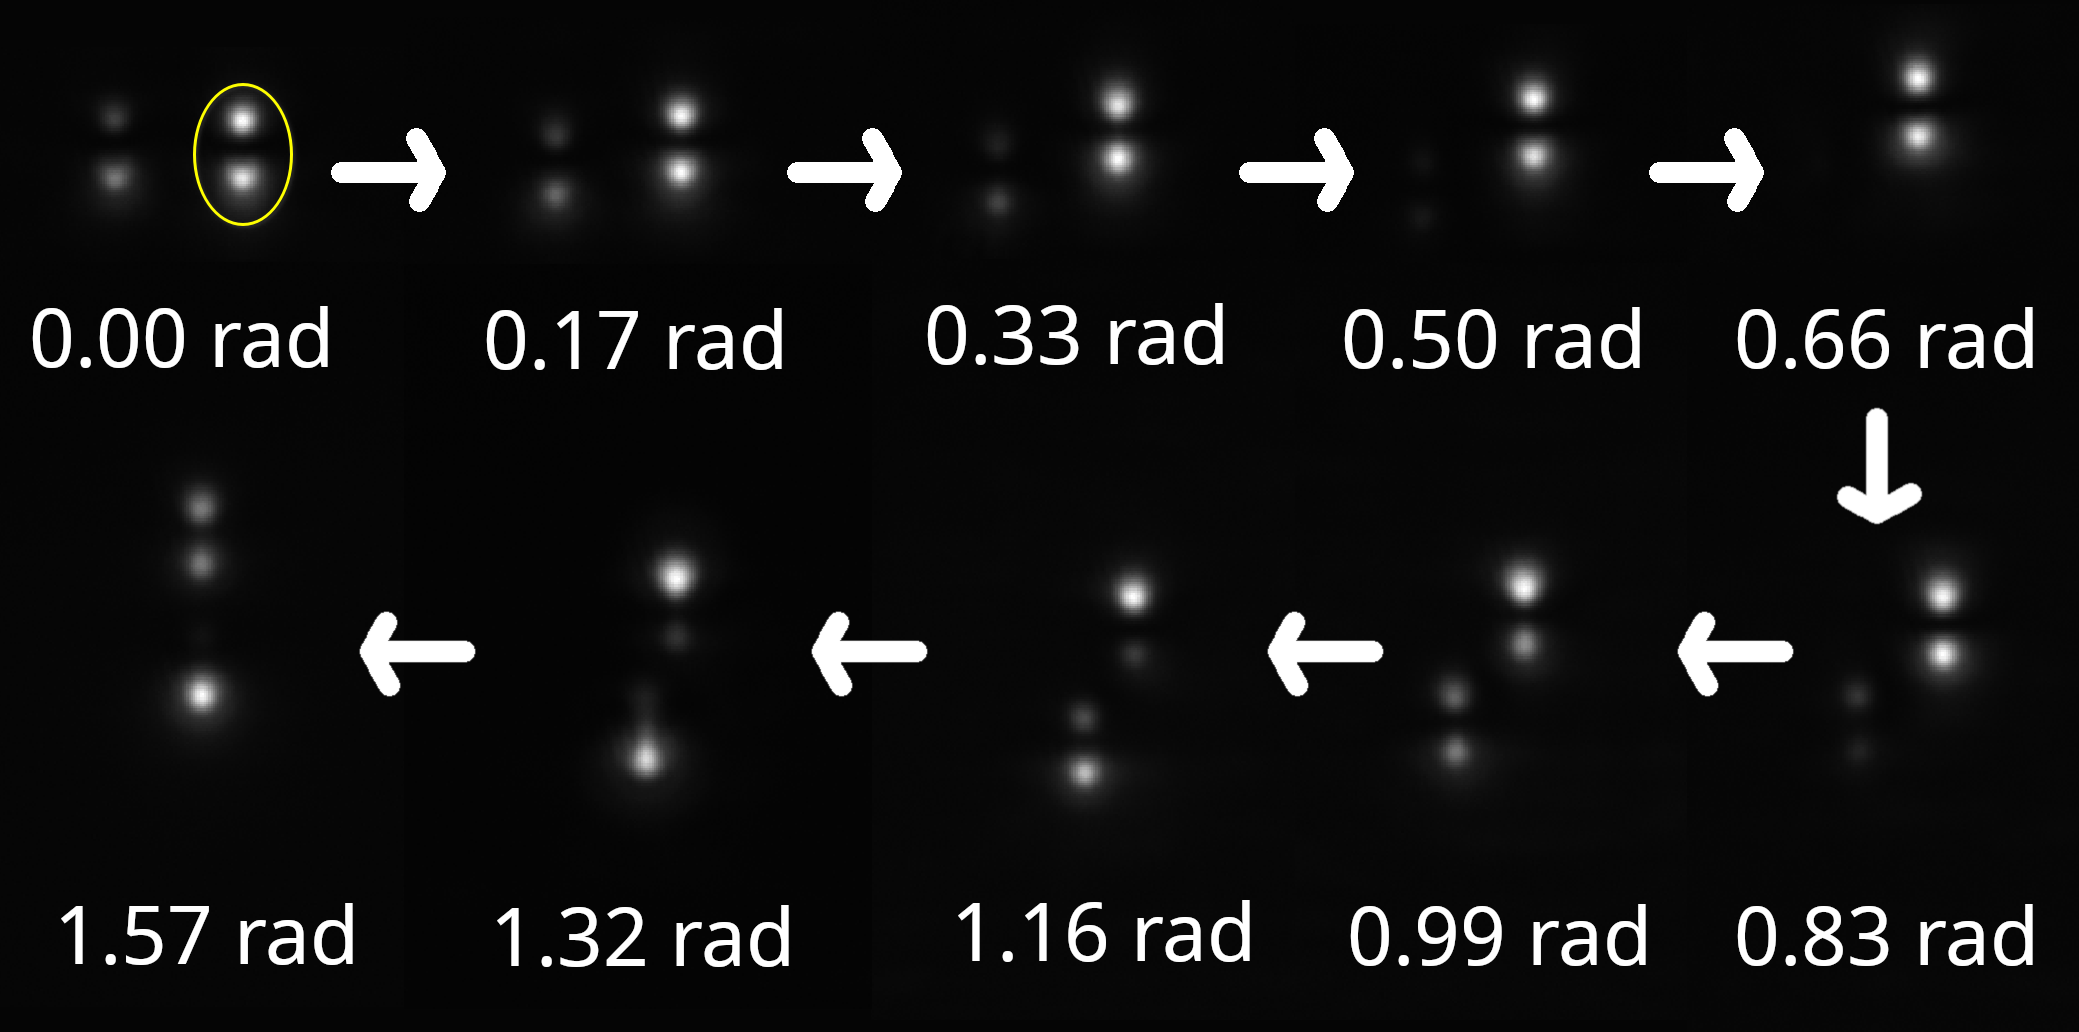
\includegraphics[trim={0 2cm 0 4cm},clip, width=\linewidth]{media/26um_15mm_angles_v2.png}
    \caption[Barrido angular experimental]{Barrido angular experimental para una distancia de propagación de 15 mm. Se observa el efecto del ángulo mágico entre 0.50 y 0.66 rad. \label{fig:angulobarrido}}
\end{figure}

Se analizaron las imágenes siguiendo el método descrito en la Sección \ref{sec:analimag}. Posteriormente, mediante la ecuación (\ref{eqn:coupling-simp}) para el acoplamiento dinámico, se caracterizó su comportamiento en función del ángulo $\theta$ (medido desde la horizontal) para una separación fija de 25 $\mu$m. El signo negativo se introdujo para garantizar la continuidad de la tendencia de los datos, como muestra la Figura \ref{fig:invisibility-coup}.

\begin{figure}[H]
    \centering
    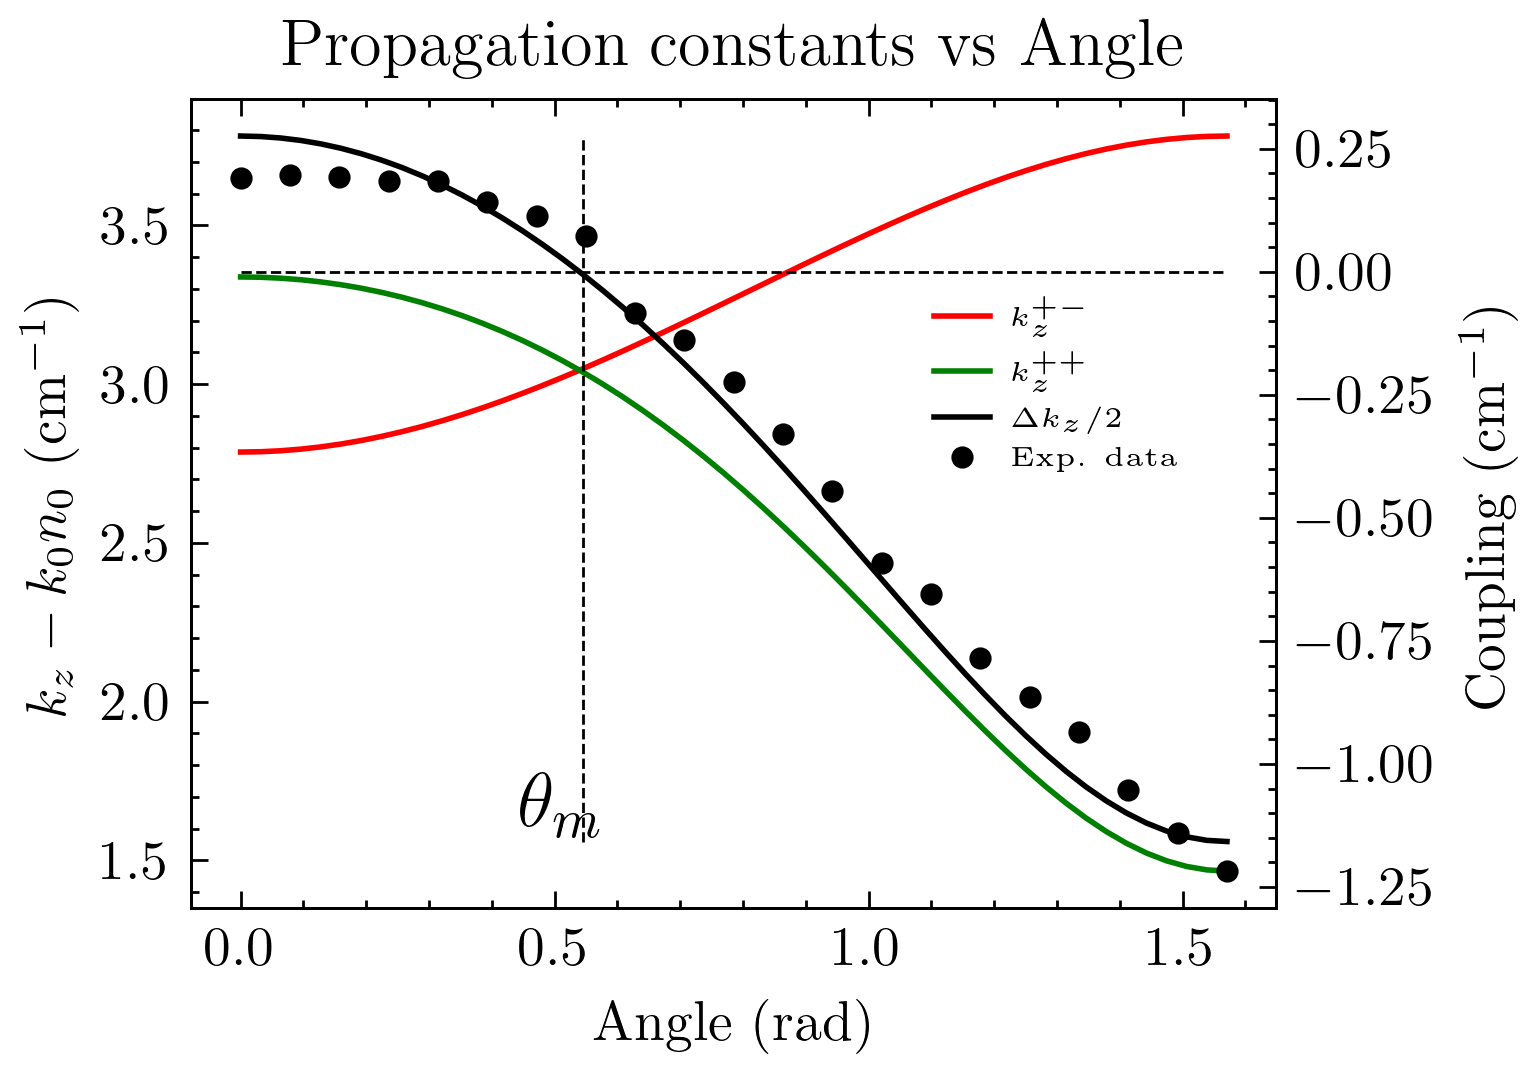
\includegraphics[width=0.7\linewidth]{codigo/eigenvalues_vs_angle.png}
    \caption[Constantes de propagación y acoplamientos angulares para modos P]{Constantes de propagación y acoplamientos en función del ángulo para modos P, calculados numéricamente mediante EME. Los resultados se comparan con los datos experimentales extraídos de la Figura \ref{fig:angulobarrido}. \label{fig:invisibility-coup}}
\end{figure}

\section{Redes tipo panal de abeja}

La red tipo panal de abeja, conocida por ser la estructura subyacente del grafeno, presenta propiedades relevantes para esta tesis, particularmente en sus bandas de Bloch: ambas son dispersivas y exhiben un punto de Dirac \citep{honeycombdirac}.

Una vez determinados los parámetros de fabricación en la sección anterior, se estudió el mismo efecto en una red tipo panal de abeja manteniendo constante la distancia entre sitios mientras se variaba el ángulo (Figura \ref{fig:HCLBW}).

\begin{figure}[H]
    \centering
    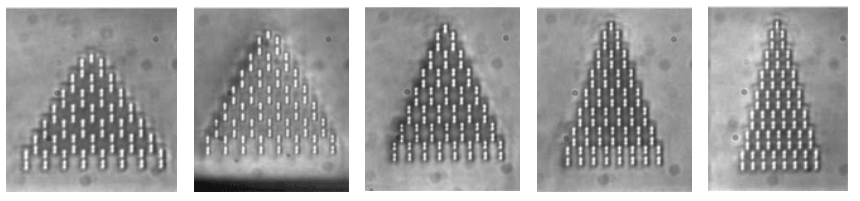
\includegraphics[width=\linewidth]{media/honeycomb_lattices_bw.png}
    \caption[Micrografías de redes fotónicas tipo panal de abeja para modos P]{Micrografías de redes fotónicas tipo panal de abeja para modos P bajo iluminación con luz blanca. \label{fig:HCLBW}}
\end{figure}

Un modelo de primeros vecinos consideraría únicamente el acoplamiento vertical $\varkappa_\sigma$ y el acoplamiento angular $\varkappa_\theta$. No obstante, la descripción precisa de los datos experimentales requiere incluir acoplamientos hasta terceros vecinos, así como correcciones por no ortogonalidad. La Figura \ref{fig:honeycombmodel} muestra un esquema del modelo completo. El Hamiltoniano del sistema se expresa como:
\begin{equation}
\hat{H}_\Sigma = \hat{H}_{NN} + \hat{H}_{NNN} + \hat{H}_{NNNN} \ ,
\end{equation}
donde $\hat{H}_{NN}$, $\hat{H}_{NNN}$ y $\hat{H}_{NNNN}$ contienen acoplamientos a primeros vecinos $\varkappa_\sigma$ y $\varkappa_\theta$, a segundos vecinos $t_\pi$ y $t_{\theta 2}$, de largo alcance $t_{\theta 1}$ y $t_{\theta 3}$, respectivamente.

{
	\sidecaptionvpos{figure}{c}
	\begin{SCfigure}[]
		\centering
		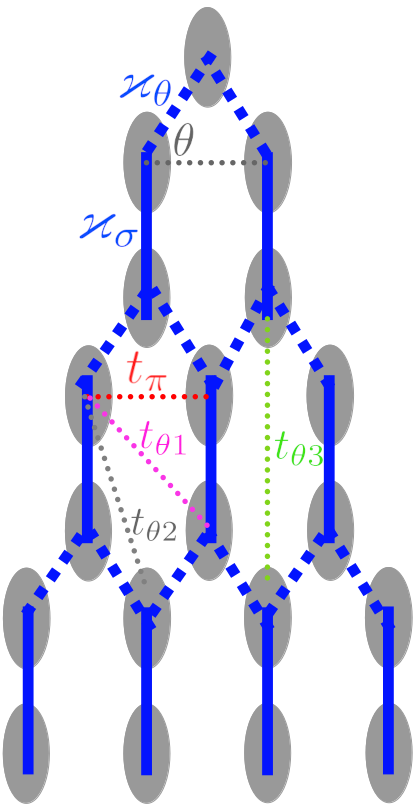
\includegraphics[width=0.25\linewidth]{media/honeycomb-lattice.png}
		\caption{Esquema del modelo de panal de abeja para modos P con acoplamientos hasta terceros vecinos. \label{fig:honeycombmodel}}
	\end{SCfigure}
}